\documentclass[a4paper,11pt,twoside]{report}
% KOMPILOWAĆ ZA POMOCĄ pdfLaTeXa, PRZEZ XeLaTeXa MOŻE NIE BYĆ POLSKICH ZNAKÓW

% -------------- Kodowanie znaków, język polski -------------

\usepackage[utf8]{inputenc}
\usepackage[MeX]{polski}
\usepackage[T1]{fontenc}
\usepackage[english,polish]{babel}

% Do poprawnego odsyłania do bibliografii i \phantomsection
\usepackage{hyperref}


\usepackage{amsmath, amsfonts, amsthm, latexsym} % głównie symbole matematyczne, środowiska twierdzeń

\usepackage[final]{pdfpages} % inputowanie pdfa
%\usepackage[backend=bibtex, style=verbose-trad2]{biblatex}

%Dla lepszego czytania list
\usepackage{blindtext}
\usepackage{enumitem}

%Do bawienia się kolorkami w grid
\usepackage{tikz}

% ---------------- Marginesy, akapity, interlinia ------------------

\usepackage[inner=20mm, outer=20mm, bindingoffset=10mm, top=25mm, bottom=25mm]{geometry}


\linespread{1.5}
\allowdisplaybreaks

\usepackage{indentfirst} % opcjonalnie; pierwszy akapit z wcięciem
\setlength{\parindent}{5mm}


%--------------------------- ŻYWA PAGINA ------------------------

\usepackage{fancyhdr}
\pagestyle{fancy}
\fancyhf{}
% numery stron: lewa do lewego, prawa do prawego 
\fancyfoot[LE,RO]{\thepage} 
% prawa pagina: zawartość \rightmark do lewego, wewnętrznego (marginesu) 
\fancyhead[LO]{\sc \nouppercase{\rightmark}}
% lewa pagina: zawartość \leftmark do prawego, wewnętrznego (marginesu) 
\fancyhead[RE]{\sc \leftmark}

\renewcommand{\chaptermark}[1]{
\markboth{\thechapter.\ #1}{}}

% kreski oddzielające paginy (górną i dolną):
\renewcommand{\headrulewidth}{0 pt} % 0 - nie ma, 0.5 - jest linia


\fancypagestyle{plain}{% to definiuje wygląd pierwszej strony nowego rozdziału - obecnie tylko numeracja
  \fancyhf{}%
  \fancyfoot[LE,RO]{\thepage}%
  
  \renewcommand{\headrulewidth}{0pt}% Line at the header invisible
  \renewcommand{\footrulewidth}{0.0pt}
}



% ---------------- Nagłówki rozdziałów ---------------------

\usepackage{titlesec}
\titleformat{\chapter}%[display]
  {\normalfont\Large \bfseries}
  {\thechapter.}{1ex}{\Large}

\titleformat{\section}
  {\normalfont\large\bfseries}
  {\thesection.}{1ex}{}
\titlespacing{\section}{0pt}{30pt}{20pt} 
%\titlespacing{\co}{akapit}{ile przed}{ile po} 
    
\titleformat{\subsection}
  {\normalfont \bfseries}
  {\thesubsection.}{1ex}{}


% ----------------------- Spis treści ---------------------------
\def\cleardoublepage{\clearpage\if@twoside
\ifodd\c@page\else\hbox{}\thispagestyle{empty}\newpage
\if@twocolumn\hbox{}\newpage\fi\fi\fi}


% kropki dla chapterów
%\usepackage{etoolbox}
%\makeatletter
%\patchcmd{\l@chapter}
%  {\hfil}
%  {\leaders\hbox{\normalfont$\m@th\mkern \@dotsep mu\hbox{.}\mkern \@dotsep mu$}\hfill}
%  {}{}
%\makeatother

%\usepackage{titletoc}
%\makeatletter
%\titlecontents{chapter}% <section-type>
%  [0pt]% <left>
%  {}% <above-code>
%  {\bfseries \thecontentslabel.\quad}% <numbered-entry-format>
%  {\bfseries}% <numberless-entry-format>
%  {\bfseries\leaders\hbox{\normalfont$\m@th\mkern \@dotsep mu\hbox{.}\mkern \@dotsep mu$}\hfill\contentspage}% <filler-page-format>

%\titlecontents{section}
%  [1em]
%  {}
%  {\thecontentslabel.\quad}
%  {}
%  {\leaders\hbox{\normalfont$\m@th\mkern \@dotsep mu\hbox{.}\mkern \@dotsep mu$}\hfill\contentspage}

%\titlecontents{subsection}
%  [2em]
%  {}
%  {\thecontentslabel.\quad}
%  {}
%  {\leaders\hbox{\normalfont$\m@th\mkern \@dotsep mu\hbox{.}\mkern \@dotsep mu$}\hfill\contentspage}
%\makeatother



% ---------------------- Spisy tabel i obrazków ----------------------

\renewcommand*{\thetable}{\arabic{chapter}.\arabic{table}}
\renewcommand*{\thefigure}{\arabic{chapter}.\arabic{figure}}
%\let\c@table\c@figure % jeśli włączone, numeruje tabele i obrazki razem


% --------------------- Definicje, twierdzenia etc. ---------------


\makeatletter
\newtheoremstyle{definition}%    % Name
{3ex}%                          % Space above
{3ex}%                          % Space below
{\upshape}%                      % Body font
{}%                              % Indent amount
{\bfseries}%                     % Theorem head font
{.}%                             % Punctuation after theorem head
{.5em}%                            % Space after theorem head, ' ', or \newline
{\thmname{#1}\thmnumber{ #2}\thmnote{ (#3)}}%  % Theorem head spec (can be left empty, meaning `normal')
\makeatother

% ----------------------------- POLSKI --------------------------------

\theoremstyle{definition}
\newtheorem{theorem}{Twierdzenie}[chapter]
\newtheorem{lemma}[theorem]{Lemat}
\newtheorem{example}[theorem]{Przykład}
\newtheorem{proposition}[theorem]{Stwierdzenie}
\newtheorem{corollary}[theorem]{Wniosek}
\newtheorem{definition}[theorem]{Definicja}
\newtheorem{remark}[theorem]{Uwaga}



% ----------------------------- Dowód -----------------------------

%\makeatletter
%\renewenvironment{proof}[1][\proofname]
%{\par
%  \vspace{-12pt}% remove the space after the theorem
%  \pushQED{\qed}%
%  \normalfont
%  \topsep0pt \partopsep0pt % no space before
%  \trivlist
%  \item[\hskip\labelsep
%        \sc
%    #1\@addpunct{:}]\ignorespaces
%}
%{%
%  \popQED\endtrivlist\@endpefalse
%  \addvspace{20pt} % some space after
%}
%
%\renewcommand{\qedhere}{\hfill \qedsymbol}
%\makeatother


% --------------------------Obrazy-----------------------------

%Path relative to the .tex file containing the \includegraphics command

\usepackage{graphicx}
\graphicspath{ {./images/} }


% -------------------------- POCZĄTEK --------------------------


% --------------------- Ustawienia użytkownika ------------------

\newcommand{\tytul}{Interfejs użytkownika do manualnego obrysu struktur oraz wybranych anormalności w obrazach medycznych z wykorzystaniem tabletu graficznego}
\renewcommand{\title}{English title}
\newcommand{\type}{inżyniers} % magisters, licencjac
\newcommand{\supervisor}{dr inż. Magdalena Jasionowska}



\begin{document}
\sloppy


\includepdf[pages=-]{titlepage}


% ---------------------------- ABSTRAKTY -----------------------------
% W PRACY PO POLSKU, NAPIERW STRESZCZENIE PL, POTEM ABSTRACT EN

{
\begin{abstract}

\begin{center}
\tytul
\end{center}

Przykładowe streszczenie. Do wykonania jako ostatnie.

\noindent \textbf{Słowa kluczowe:} slowo1, slowo2, ...
\end{abstract}
}

\null\thispagestyle{empty}\newpage

{
\selectlanguage{english}
\begin{abstract}

\begin{center}
\title
\end{center}

Sample abstract in english.

\noindent \textbf{Keywords:} keyword1, keyword2, ...
\end{abstract}
}


% --------------------- OŚWIADCZENIE -----------------------------------------


\null\thispagestyle{empty}\newpage

\null \hfill Warszawa, dnia ..................\\

\par\vspace{5cm}

\begin{center}
Oświadczenie
\end{center}

\indent Oświadczam, że moją część pracy \type kiej (zgodnie z podziałem zadań opisanym na wstępie) pod
tytułem ,,\tytul '', której promotorem jest \supervisor , wykonałem
samodzielnie, co poświadczam własnoręcznym podpisem.
\vspace{2cm}


\begin{flushright}
  \begin{minipage}{50mm}
    \begin{center}
      ..............................................

    \end{center}
  \end{minipage}
\end{flushright}

\thispagestyle{empty}
\newpage

\null\thispagestyle{empty}\newpage


% ------------------- 4. Spis treści ---------------------
\pagenumbering{gobble}
\tableofcontents
\thispagestyle{empty}

%\newpage % JEŻELI SPIS TREŚCI MA PARZYSTĄ LICZBĘ STRON, ZAKOMENTOWAĆ
% ALBO JAK KTOŚ WOLI WTEDY DWIE STRONY ODSTĘPU, DODAĆ \null\newpage

% -------------- 5. ZASADNICZA CZĘŚĆ PRACY --------------------
\null\thispagestyle{empty}\newpage
\pagestyle{fancy}
\pagenumbering{arabic}
\setcounter{page}{11} % JEŻELI Z POWODU DUŻEJ ILOŚCI STRON W SPISIE TREŚCI SIĘ NIE ZGADZA, TRZEBA ZMODYFIKOWAĆ RĘCZNIE
%oryginalnie było 11
%ustawiam ponownie 11, usunąłem pustą stronę po spisie treści - rodziały powinny zaczynać się na stronach nieparzystych

\chapter*{Wstęp}
\markboth{}{Wstęp}
\addcontentsline{toc}{chapter}{Wstęp}

O czym jest praca? Co się w niej znajduje? Jaki jest wkład autora?

\chapter {Wprowadzenie}

\section {Zagdanienia medyczne związane z aplikacją}

\section {Podział prac}


\chapter {Stan wiedzy}

W poniższym rozdziale zostały przestawione istniejące na rynku aplikacje oferujące podobne funkcjonalności do wymagań postawionych przed autorskim systemem do obrysów na obrazach DICOM. Przedstawiono również proponowane rozwiązanie postawionych przed systemem wymagań.

\section {Przegląd istniejących rozwiązań}

\subsection {Cornerstone}

Cornerstone Core to biblioteka, która umożliwia wyświetlanie obrazów medycznych z wykożystaniem elementu canvas z języka HTML5. Biblioteka udostępnia interfejs do wyświetlania obrazów medycznych pozwalający na zarządzanie wyświetlaniem zdjęcia. Podstawowe funkcjonalności obsługiwane przez bibliotekę to:

\begin{itemize}[noitemsep]
\item Przybliżanie i oddalanie obrazu.
\item Obrót obrazu.
\item Przesuwanie obrazu w wyświetlanym komponencie.
\item Zmiana jasności wyświetlanego obrazu.
\item Mapowanie kolorów.
\item Interpolacja pikseli w obrazie (dla obrazów o niskiej rozdzielczości).
\end{itemize}

Ponadto twórcy biblioteki Cornerstone Core stworzyli bibliotekę Cornerstone Tools, która korzysta z biblioteki Cornerstone Core i umożliwia wiele funkcjonalności potrzebnych lekarzom do analizy badań pacjentów. Poza funkcjonalnościami Cornerstone Core umożliwia także:

\begin{itemize}[noitemsep]
\item Mierzenie odległości w linii prostej na obrazie z podaniem rzeczywistych wartości.
\item Oznaczanie obszarów przy pomocy prostokątów oraz elips.
\item oznaczanie niewielkich zmian w postaci małego okręgu.
\item Mierzenie kątów na podstawie 3 podanych przez użytkownika punktów.
\end{itemize}

Przykładowym projektem korzystającym z bibliotek Cornerstone jest OHIF\footnote {Open Health Imaging Foundation - http://ohif.org/ } Viewer. Aplikacja pozwala na wykorzystanie większości możliwości udostępnianych przez biblioteki Cornerstone. Przykładowe urzycie aplikacji zostało przedstawione na rysunku \ref{fig:OHIF-example}.

\begin{figure}[h]
	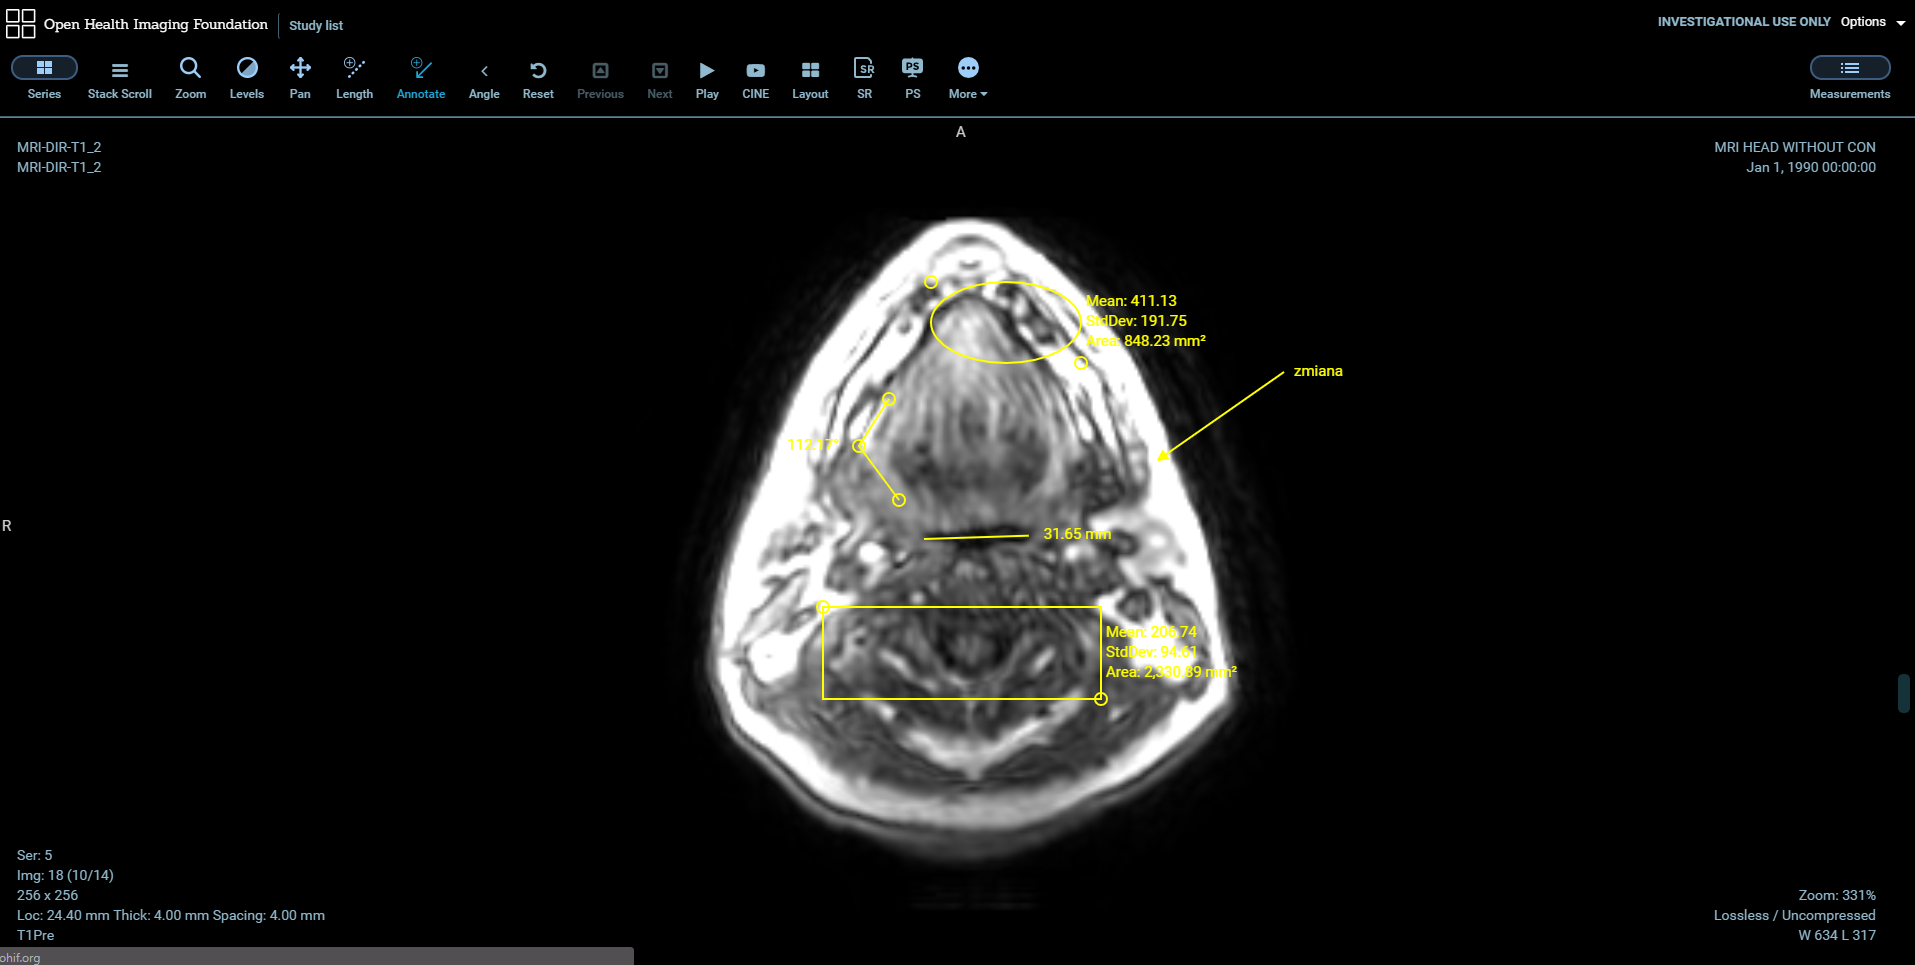
\includegraphics[width=\textwidth]{OHIF-example}
	\caption{Przykład użycia aplikacji OGIF Viewer}
    	\label{fig:OHIF-example}
\end{figure}

\subsection {DICOM Web Viewer (DWV)}
\subsection {Dicom-contour}
\subsection {Orthanc}

Orthanc to serwer z bazą plików DICOM, który umożliwia łatwe przechowywanie, zarządzanie oraz dostęp do plików medycznych DICOM. Ponadto Orthanc udostępnia REST API, które umożliwia przeglądanie wgranych na serwer plików DICOM podzielonych względem pacjentów, badań i serii. 

Serwer Orthanc udostępnia również prosty interfejs przeglądarkowy który pozwala na wgrywanie nowych plików (interfejs wgrywania plików przedstawiono na ryskunku \ref{fig:Orthanc-upload}), przeglądanie zapisanych plików --- w szczególności tagów (rysunek \ref{fig:Orthanc-tags}) oraz podglądu obrazu (rysunek \ref{fig:Orthanc-preview}). Interfejs przeglądarkowy nie zapewnia żadnej metody rysowania na przeglądanym obrazie. Pozwala natomiast na przełączanie obrazu na kolejny lub poprzedni poprzez kliknięcie lewym przyciskiem myszy w prawą lub część podglądu obrazu.

\begin{figure}[h]
	\center
	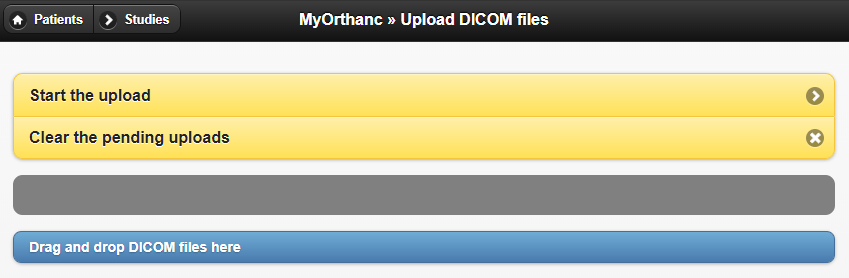
\includegraphics[width=0.8\textwidth]{Orthanc-upload}
	\caption{Interfejs wgrywania plików DICOM do serwera Orthanc}
    	\label{fig:Orthanc-upload}
\end{figure}

\begin{figure}[h]
	\center
	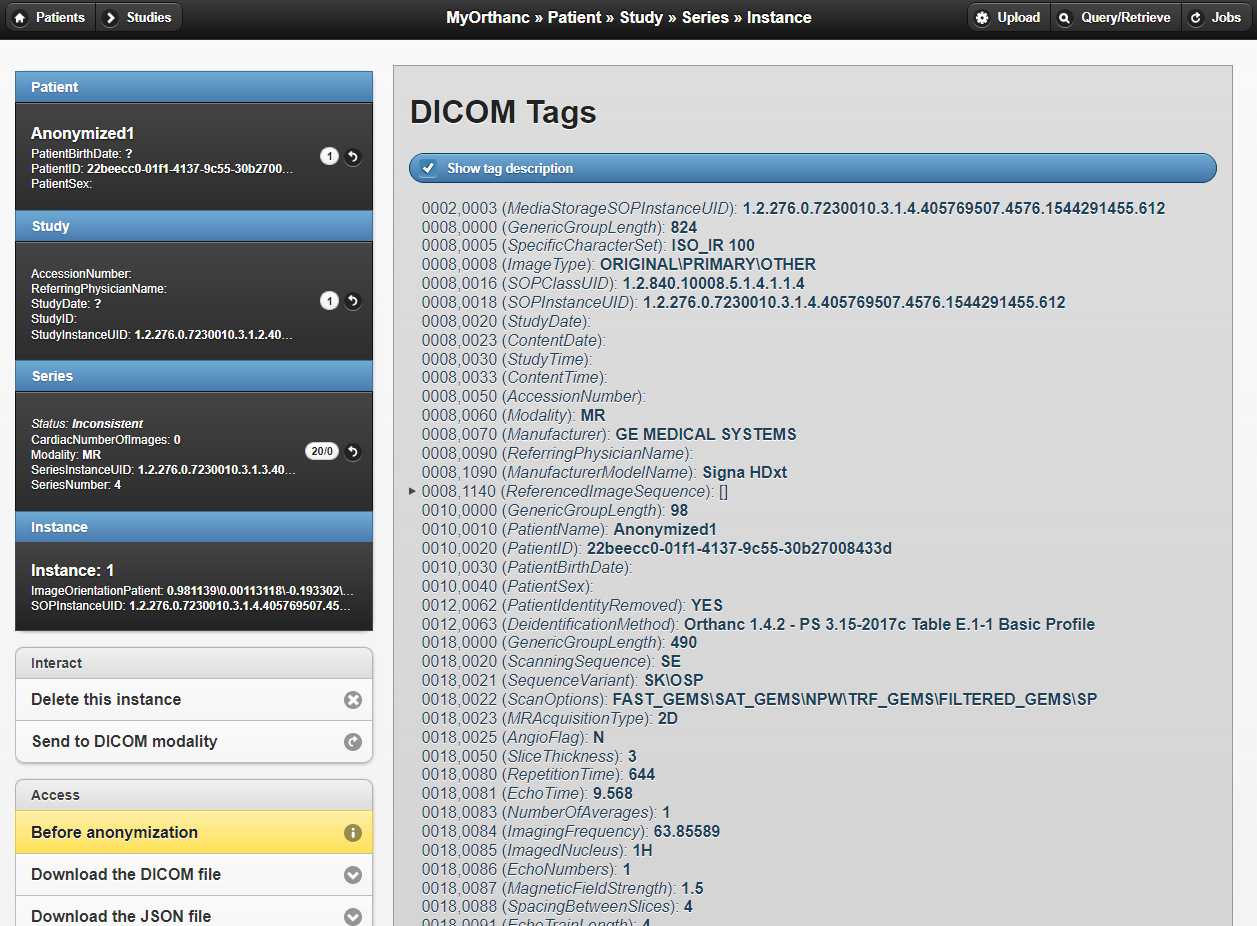
\includegraphics[width=0.8\textwidth]{Orthanc-tags}
	\caption{Podgląd tagów pliku DICOM przez interfejs przeglądarkowy Orthanc}
    	\label{fig:Orthanc-tags}
\end{figure}

\begin{figure}[h]
	\center
	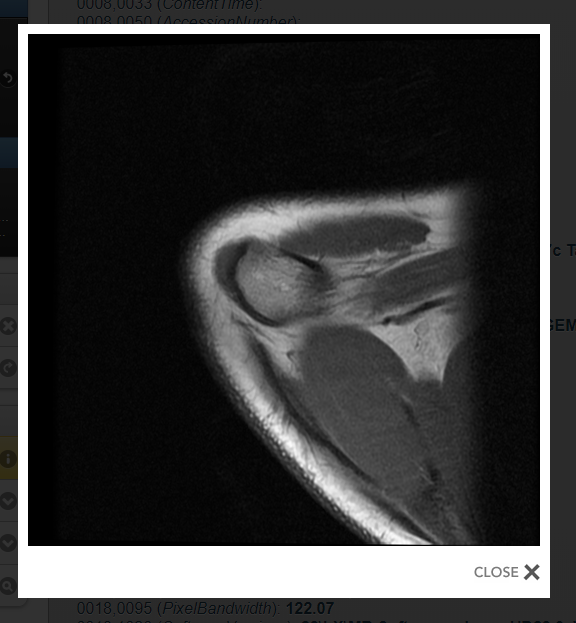
\includegraphics[width=0.8\textwidth]{Orthanc-preview}
	\caption{Podgląd obrazu DICOM przez interfejs przeglądarkowy Orthanc}
    	\label{fig:Orthanc-preview}
\end{figure}

\section {Proponowane rozwiązanie}


\chapter {Opis autorskiego systemu informatycznego}

W poniższym rozdziale zawarto dokumentację techniczną i biznesową tworzonego systemu. Przedstawiono w szczególności: wymagania, architekturę, zastosowane metody półautomatycznego obrysu oraz metody obliczania statystyk obrysu.

\section {Specyfikacja wymagań}

\subsection {Opis biznesowy}

Celem projektu jest stworzenie interfejsu przyjaznego użytkownikowi, który umożliwi przeglądanie plików DICOM, a także przeprowadzanie na tych plikach obrysów. Prace obejmują stworzenie aplikacji webowej, która udostępni użytkownikowi interfejs komunikujący się z bazą danych Orthanc oraz serwera odpowiedzialnego za przechowywanie wygenerowanych przez użytkownika obrysów oraz wyznaczanie obrysów półautomatycznych. 

Do podstawowych funkcjonalności systemu zaliczają się:
\begin{itemize}[noitemsep]
%O listach wyliczeniowych https://sjp.pwn.pl/poradnia/haslo/listy-wyliczeniowe;4812.html
\item Generowanie obrysu manualnego.
\item Generowanie obrysu półautomatycznego na podstawie punktów podanych przez użytkownika.
\item Zapisywanie wygenerowanych obrysów.
\item \textbf {Anonimizacja}\footnote {Anonimizacja (ang. anonymization) --- operacja mająca na celu usunięcie z danych informacji o pacjentach, które pozwoliłyby na identyfikację danych z tożsamością pacjenta. Są to między innymi: imiona, nazwisko, pesel. Inne tłumaczenia słowa anonymization --- utajnianie, usuwanie danych niejawnych. Z uwagę na fakt, że te tłumaczenia nie oddają dobrze kontekstu zastosowano kalkę językową.} danych zapisanych w strukturze pliku DICOM.
\end{itemize}

\subsection {Wymagania funkcjonalne}

Poniżej przedstawiono wymagania funkcjonalne w postaci historyjek użytkownika (ang. user stories): 
\begin{enumerate}
\item \textbf {Jako użytkownik chcę wczytać obraz DICOM.} \\
Użytkownik może wybrać obraz w menu bocznym, w którym ma możliwość wyboru pacjenta, badania oraz serii. Wybranie serii skutkuje wyświetleniem pierwszego obrazu DICOM z tej serii.

\item \textbf {Jako użytkownik chcę zmienić obraz w serii przy użyciu rolki myszy.} \\
Po najechaniu na obraz przewijanie rolką myszy do góry powoduje zmianę wyświetlanego obrazu na kolejny obraz w serii. Gdy przewijamy rolką myszy do góry na ostatnim obrazie w serii wyświetlany obraz nie zmienia się. Analogicznie przewijanie rolką myszy w dół powoduje zmianę wyświetlanego obrazu na poprzedni obraz w serii, a przewijanie w dół rolką myszy na pierwszym obrazie w serii nie powoduje zmiany obrazu.

\item \textbf {Jako użytkownik chcę wykonać obrys przy użyciu tabletu graficznego.} \\
Po najechaniu na obraz kursorem sterowanym przez tablet graficzny, po wciśnięciu końcówki rysika użytkownik prowadzi kursor po obrazie wykonując obrys bez odrywania końcówki rysika od podkładki. Jeżeli użytkownik nie zakończy obrysu dokładnie w punkcie, w którym go rozpoczął, obrys powinien zakończyć się linią prostą, łączącą punkt końcowy z punktem początkowym.

\item \textbf {Jako użytkownik chcę wygenerować obrys na podstawie wybranych punktów.} \\
Po najechaniu kursorem na obraz użytkownik może wybierać punkty, na podstawie których zostanie wygenerowany obrys, poprzez wciśnięcie lewego przycisku myszy w miejscach, w których chce, aby znalazły się punkty. Użytkownik może zobaczyć efekt wygenerowanego przez system obrysu

\item \textbf {Jako użytkownik chcę edytować listę punktów, z której wygenerowany zostanie obrys.} \\
Użytkownik może usunąć wcześniej wybrany punkt po najechaniu na niego kursorem i wciśnięciu lewego przycisku myszy. Użytkownik może dodać nowy punkt do listy punktów poprzez wciśnięcie lewego przycisku myszy w miejscu, w którym chce wstawić punkt.

\item \textbf {Jako użytkownik chcę wybrać kolor obrysu.} \\
Użytkownik wybiera kolor z palety kolorów lub zdefiniować własny kolor poprzez podanie numeru RGB koloru, który chce wybrać.

\item \textbf {Jako użytkownik chcę zapisać obrys.} \\
Po wykonaniu obrysu manualnego lub wybraniu listy punktów do wygenerowania obrysu półautomatycznego użytkownik wybiera nazwę obrysu i zapisuje obrys w systemie.

\item \textbf {Jako użytkownik chcę obejrzeć zapisany obrys.} \\
Użytkownik wybiera z listy po prawej stronie zapisany obrys i przegląda obrys naniesiony na obraz, na którym został wykonany.

\item \textbf {Jako użytkownik chcę zobaczyć statystyki dotyczące obrysu.} \\
Użytkownik wybiera z listy po prawej stronie zapisany obrys i przegląda statystyki obliczone na podstawie zapisanego obrysu. Do statystyk zalicza się obwód obrysu, pole obrysu, histogram obrazu na obszarze obrysu oraz liczba pikseli wewnątrz obrysu.

\item \textbf {Jako użytkownik chcę zobaczyć jednocześnie dowolną liczbę zapisanych w systemie obrysów na jednym obrazie DICOM.} \\
Użytkownik wybiera poprzez kliknięcie lewym przyciskiem myszy na nazwie obrysu znajdującej się na liście po prawej stronie. Wybrane obrysy wyświetlane są jednocześnie na przeglądanym przez użytkownika zdjęciu. Użytkownik może wyłączyć podgląd wcześniej wybranego obrysu poprzez ponowne wciśnięcie lewego przycisku myszy na nazwie obrysu na liście po prawej stronie. Na zdjęciu wyświetlane są jedynie obrysy wykonane na tym obrazie.

\item \textbf {Jako użytkownik chcę zanonimizować dane pacjenta zawarte w pliku DICOM.} \\
Użytkownik może zanonimizować pacjenta, gdy przegląda jego obraz. Użytkownik może anonimizować imię i nazwisko pacjenta, datę urodzenia pacjenta oraz płeć pacjenta poprzez nadanie nowych wartości lub poprzez usunięcie poprzedniej wartości i pozostawienie pustych pól w formularzu.

\end{enumerate}

\subsection {Wymagania niefunkcjonalne}

%\begin{table}[b!]{ c | l | p } % Koniecznie label po caption, inaczej jest zła numeracja
%\caption[Opis skrócony]{Spis wymagań niefunkcjonalnych}
%\label{tabela wymagania niefunkcjonalne}
%\centering
%\begin{tabular}
%Obszar wymagań & Nr wymagania & Opis \\ \hline
%1 & 2 & 3 
%\end{tabular}
%\end{table}

\begin{table}
\caption[Opis skrócony]{Spis wymagań niefunkcjonalnych}
\label{tabela wymagania niefunkcjonalne}
\centering
\begin{tabular}{ | p{0.2\textwidth} | p{0.15\textwidth} | p{0.5\textwidth} | }
\hline
  Obszar wymagań & Nr wymagania & Opis \\ \hline
  Użyteczność (ang. Usability) & 1 & Każda funkcjonalność aplikacji dostępna dla użytkownika musi mieścić się na pojedynczym ekranie przy rozdzielczości 1920x1080 i czcionce nie mniejszej niż 12pt. \\ 
  \cline{2-3}
    & 2 & Aplikacja powinna udostępniać pobranie zapisanych obrysów przy użyciu serwisu REST. \\ \hline
  Niezawodność (ang. Reliability) & 3 & Aplikacja ma być dostępna 24h w ciągu doby. Dopuszczalne jest brak działania aplikacji w dowolnym momencie przez okres nie dłuższy niż przez 12h. Po przerwie w działaniu aplikacja musi być dostępna przez kolejne 24h bez utrudnień. \\ \hline
  Wydajność (ang. Performance) & 4 & Aplikacja powinna pobierać dane zewnętrzne w postaci pliku DICOM (około 20MB) nie dłużej niż 5 sekund \\ 
  \cline{2-3}
  & 5 & Aplikacja powinna generować obrys półautomatyczny i zapisywać obrys do systemu w czasie nie dłuższym niż 30 sekund. \\ 
  \cline{2-3}
  & 6 & Aplikacja powinna reagować na działanie użytkownika (z wyłączeniem generowania obrysu półautomatycznego i zapisu obrysu do systemu) w czasie nie dłuższym niż 1 sekunda. \\
  \hline
\end{tabular}
\end{table}

Tabela \ref{tabela wymagania niefunkcjonalne} przedstawia wymagania niefunkcjonalne, które system musi spełnić.

\section {Architektura rozwiązania}

\section {Opracowany algorytm półautomatyczny}

Opracowany algorytm półautomatyczny służy do wykrywania krawędzi na obrazie medycznym. Jest algorytmem półautomatycznym, ponieważ jest wspomagany przez człowieka --- użytkownika, który wybiera punkty na ekranie. Te punkty są interpolowane przez algorytm półautomatyczny, zwany dalej algorytmem.

Jako dane wejściowe do algorytmu uzyskujemy następujące informacje:
\begin{itemize}[noitemsep]
\item {Identyfikator obrazu medycznego, na którym był wykonywany obrys.}
\item {Lista punktów wybranych przez użytkownika. Punkty te zostały wcześniej przeskalowane ze współrzędnych w aplikacji internetowej (aplikacji webowej, ang. web application) na współrzędne odpowiadające rozdzielczości obrazu medycznego.}
\end{itemize}


Algorytm można podzielić na kilka ważnych etapów:

\begin{itemize}[noitemsep]
\item {Wykrycie krawędzi na bitmapie,}
\item {Stworzenie grafu z bitmapy,}
\item {Zapewnienie spójności grafu,}
\item {Wyszukanie najkrótszych ścieżek w grafie.}
\end{itemize}

Poniżej zostaną przedstawione dokładne rozwiązania dla każdego z tych kroków. Przed rozpoczęciem przetwarzania jest pobierany obraz medyczny o danym wcześniej identyfikatorze ze serweru Orthanc. Jest on podstawą do dalszej pracy algorytmu.


\subsection {Wykrycie krawędzi na bitmapie}

Często na obrazach medycznych różnice w charakterystyce poziomów szarości pikseli reprezentujących interesujące nas obiekty są małe, nie są dane dodatkowe informacje o naturze obrazu. Problem opracowania uniwersalnego algorytmu wykrywania krawędzi jest problemem trudnym. Dla wielu algorytmów można znaleźć takie przykłady, że te algorytmy nie wyznaczą poprawnie krawędzi. Ponadto są wymagania dla stwierdzania poprawności działania danego algorytmu, czy też operatora morfologicznego. Zgodnie z \cite{Cyfrowe przetwarzanie obrazów medycznych} ,,dobry detektor krawędzi powinien spełniać następujące warunki:
\begin{itemize}[noitemsep]
\item {niskie prawdopodobieństwo zaznaczenia punktów nienależących do krawędzi oraz niskie prawdopodobieństwo niezaznaczenia punktów należących do krawędzi,}
\item {zaznaczone pukty krawędzi powinny być możliwie blisko jej osi,}
\item {wyłącznie jedna odpowiedź na pojedyńczy punkt krawędzi.''}
\end{itemize}

Po zapoznaniu się z literaturą związaną z przetwarzaniem obrazów medycznych w algorytmie został użyty operator Canny'ego. Jest on powszechnym i dobrze sprawdzonym rozwiązaniem do wykrywania krawędzi. Jak napisał autor \cite{Cyfrowe przetwarzanie obrazów medycznych} ,,Operator ten (Canny'ego) jest bardzo popularny, chętnie wykorzystywany i adoptowany do wielu zastosowań. (\dots) Stał on się również standardem często używanym do porównań innych metod wykrywania krawędzi.'' Zgodnie z rysunkiem 4.25 ,,Porównanie operatorów wykrywania krawędzi'' w \cite{Cyfrowe przetwarzanie obrazów medycznych} najlepiej wykrywał główne narządy, takie jak wątroba czy też trzustka. Z wyżej wymienionych powodów został on wykorzystany w tym algorytmie.

Operator Canny'ego \cite{Canny} składa się z 3 zasadniczych kroków:
\begin{enumerate}%[noitemsep]
\item \textbf {Określenie wartości i kąta gradientu.} \\
W tym celu został wykorzystany operator gradientu, a estymatorem gradientu w funkcji dyskrentej, jaką jest obraz zastosowano maskę, czy też operator Sobela. Wykorzystując go uzskano dla każdego piksela wielkość oraz kierunek gradientu, co służy do dalszych obliczeń. 
\item \textbf {Wykrycie miejsc występowania krawędzi.} \\
W tym celu został wykorzystany algorytm non-max suppression. Polega on na wyborze takich pikseli, które mają największą wartość gradientu na linii o kierunku zgodnym z kątem danego gradientu. Możliwe są 4 kierunki: pionowy, poziomy oraz dwa diagonalne. Jeśli dany piksel miał większą wartość gradientu od dwóch swoich sąsiadów, to zaznaczono go jako potencjalny punkt tworzący krawędzie. W ten sposób otrzymano obraz z potencjalnymi krawędziami.
\item \textbf {Wyznaczanie krawędzi progowaniem histerezy} \\
Po poprzednim kroku na obrazie nadal znajdują się nieistotne krawędzie. W tym celu Canny wprowadził ideę progowania histerezy. Metoda ta wymaga 2 wartości progowych $T_1, T_2$ takich, że $T_1 < T_2$. Jeżeli wartość gradientu w danym pikselu jest większa od $T_2$, to zaznaczono ten punkt jako krawędź. Jeśli tak się stało, to zaczęto proces śledzenia krawędzi --- dla każdego sąsiada, którego wartość gradientu jest większa od $T_1$ zaznaczono go jako krawędź. Jest ona wykonywana rekurencyjnie dla każdego zakwalifikowanego punktu. 

Zamiast dokładnych wartości progowych można przekazać do funkcji 2 wartości --- $t_1, t_2$, które są procentem liczby pikseli, które będą niedopuszczone jako krawędzie. Dla $t_1 = 0.7, t_2 = 0.9$ dopuszczono tylko 10\% pikseli jako te, które są większe od $T_2$. Podając $t_1, t_2$ wyznaczono rozkład wartości gradientu w badanym obrazie, obliczono dystrybuantę $F(x)$ i wybrano dla $T_1$ ten argument, dla którego $F(x) = t_1 * liczba pikseli$ i analogicznie dla $T_2$. W ten sposób wyznaczono progi do histerezy.

\end{enumerate}

Operator Sobela \cite{Sobel} to metoda wyznaczania gradientu, a więc zarazem krawędzi zarówno w kierunku poziomym, jak i w pionowym. Dla każdego piksela przeprowadzono operację morflologiczną z następującymi maskami:

\begin{table}[h!]
\centering
\begin{tabular} { c c }
  Maska rzędów & Maska kolumn \\ 
$
\begin{matrix}
-1 & -2 & -1 \\
0 & 0 & 0 \\
1 & 2 & 1
\end{matrix}$
&
$\begin{matrix}
-1 & 0 & 1 \\
-2 & 0 & 2 \\
-1 & 0 & 1
\end{matrix}$
\end{tabular}
\end{table}

Po wykonaniu tych operacji otrzymano wartości $s_1$ i $s_2$ odpowiednio dla maski rzędów i kolumn. Na podstawie tych danych otrzymano następujące informacje o gradiencie:
\begin{table}[h!]
\centering
\begin{tabular} { c c }
  Wielkość gradientu & Kierunek krawędzi \\ 
$\sqrt{s_1^2 + s_2^2}$ & $\tan^{-1} \Bigg[ {\cfrac{s_1}{s_2}} \Bigg]$
\end{tabular}
\end{table}

Detektory krawędzi oparte na gradiencie, w tym operator Canny'ego są często używane. Za ich główne zalety na podstawie \cite{Cyfrowe przetwarzanie obrazów medycznych} są:
\begin{itemize}[noitemsep]
\item Dają dobre wyniki dla obrazów o dobrej jakości i bez szumów.
\item Są wydajne - ich złożoność jest liniowa względem liczby przetwarzanych pikseli.
\item Nie wymagają skomplikowanej sztucznej inteligencji do działania.
\end{itemize}

Zgodnie z \cite{Cyfrowe przetwarzanie obrazów medycznych} za ich główne wady można uznać:
\begin{itemize}[noitemsep]
\item ,,Konieczność określenia rozmiaru maski i wartości progowej. Rozmiar maski znacząco wpływa na położenie miejsc, w których gradient przecina zera lub osiąga wartości maksymalne.
\item Pomijanie narożników spowodowane faktem, że wartość 1D gradientu w narożnikach jest zwyczajnie mała.
\item Operator pierwszej pochodnej wykrywa tylko schodkowe krawędzie.
\item Duża wrażliwość na szum.''
\item Na podstawie obserwacji działania algorytmu - rozmyte krawędzie często nie są wykrywane przez małe różnice w wartościach kolejnych sąsiadujących pikseli.
\end{itemize}

W ten sposób otrzymano macierz, gdzie każde pole w macierzy odpowiada pikselowi w wejściowej bitmapie --- obrazie medycznym. Jeśli w komórce macierzy znajduje się 1, to w tym miejscu na bitmapie znajduje się krawędź, w przeciwnym przypadku 0. W ten sposób algorytm wykrył wszystkie znaczące krawędzie na bitmapie. Kolejnym krokiem przetwarzania było stworzenie grafu na podstawie wyżej wymienionej macierzy.

\subsection {Stworzenie grafu z bitmapy}

Na tym etapie algorytm potrzebuje następujących danych wejściowych:
\begin{itemize}[noitemsep]
\item Macierz z wartościami logicznymi prawda/fałsz czy znajduje się danym punkcie krawędź. Może to być także realizowane poprzez macierz wartości liczbowych.
\item Punkty wybrane przez użytkownika aplikacji.
\end{itemize}

%Jaki tutaj -? - czy --?
Przed rozpoczęciem działania algorytmu należy zapewnić łączność 4-krotną (ang. Pixel 4-connectivity) \cite{Pixel connectivity}. Jest ona zwana także sąsiedztwem von Neumanna. Przy łączności 4-krotnej sprawdza się tylko sąsiadów w poziomie lub pionie.

%Opisać te rysunki i wywalić stąd - nie muszą być dokładnie w tym miejscu.
\begin{center}
\begin{tikzpicture}
\draw[step=1cm,gray,very thin] grid (3,3);
\fill[fill=black!60!white, draw=black] (1,1) rectangle (2,2);
\fill[fill=gray!60!white, draw=black] (1,0) rectangle (2,1);
\fill[fill=gray!60!white, draw=black] (0,1) rectangle (1,2);
\fill[fill=gray!60!white, draw=black] (2,1) rectangle (3,2);
\fill[fill=gray!60!white, draw=black] (1,2) rectangle (2,3);
\end{tikzpicture}
\end{center}

Dla łączności 8-krotnej sprawdza się wszystkich możliwych sąsiadów, także po przekątnej. Jest ona zwana także sąsiedztwem Moore'a lub otoczeniem Moore'a \cite{Moore}.

\begin{center}
\begin{tikzpicture}
\draw[step=1cm,gray,very thin] grid (3,3);
\fill[fill=black!60!white, draw=black] (1,1) rectangle (2,2);
\fill[fill=gray!60!white, draw=black] (1,0) rectangle (2,1);
\fill[fill=gray!60!white, draw=black] (0,1) rectangle (1,2);
\fill[fill=gray!60!white, draw=black] (2,1) rectangle (3,2);
\fill[fill=gray!60!white, draw=black] (1,2) rectangle (2,3);
\fill[fill=gray!60!white, draw=black] (0,0) rectangle (1,1);
\fill[fill=gray!60!white, draw=black] (2,2) rectangle (3,3);
\fill[fill=gray!60!white, draw=black] (0,2) rectangle (1,3);
\fill[fill=gray!60!white, draw=black] (2,0) rectangle (3,1);
\end{tikzpicture}
\end{center}

%Bibliografia do tego?
W przypadku zastosowania łączności 8-krotnej przy wyznaczaniu długości krawędzi musiano by zastosować metrykę Czebyszewa, która jest specjalnym przypadkiem odległości Minkowskiego. Jeśli zostanie łączność 4-krotna to długość krawędzi byłaby obliczana zgodnie z metryką miejską, zwaną też metryką Manhattan. 

Metryka Manhattan w kontekście dalszego przetwarzania w celu wyszukiwania najkrótszych ścieżek w grafie jest bardziej adekwatna, ponieważ jest intuicyjna w wyznaczaniu odległości na obrazie płaskim w porównaniu do metryki Czebyszewa. W tym przypadku najlepsza byłbay tutaj metryka Euklidesa, lecz mamy do czynienia nie z kolejnymi punktami oddalonymi od siebie, a z sąsiadującymi pikselami. Ponadto w tym algorytmie istotne jest szybkie szacowanie odległości, czy też długości danej krawędzi.

Wykrywanie wierzchołków przy łączności 4-krotnej jest prostsze. Wystarczy zliczyć liczbę sąsiadów. Poniżej zakładamy, że piksel jest oznaczony jako krawędź w macierzy wejściowej. W zależności od liczby sąsiadów mamy następujące przypadki:
\begin{itemize}[noitemsep]
\item 0 --- wierzchołek izolowany,
\item 1 --- punkty końcowe (ang. endpixels),
\item 2 --- punkty łączące (ang. linkpixels), czyli fragmenty krawędzi,
\item 3--4 --- punkty węzłowe (ang. vertices), czyli punkty, od których odchodzą co najmniej 3 krawędzie.
\end{itemize}

W przypadku łączności 8-krotnej do detekcji wierzchołków należałoby stosować przekształcenia Hit-or-Miss z elementami strukturalnymi. Elementy strukturalne do wykrywania odpowiednich punktów są następujące:
\begin{itemize}%[noitemsep]
\item wierzchołek izolowany: \\
$
\begin{bmatrix}
0 & 0 & 0 \\
0 & 1 & 0 \\
0 & 0 & 0 
\end{bmatrix}
$,
\item punkty końcowe (ang. endpixels): \\
$
\begin{bmatrix}
0 & 0 & 0 \\
0 & 1 & 0 \\
z & z & z 
\end{bmatrix}
$,
\item punkty łączące (ang. linkpixels), czyli fragmenty krawędzi, posiadają dokładnie 2 sąsiadów,
\item punkty węzłowe (ang. vertices), czyli punkty, od których odchodzą co najmniej 3 krawędzie: \\
$
\begin{bmatrix}
z & 1 & z \\
z & 1 & z \\
z & z & 1 
\end{bmatrix}
$ lub $
\begin{bmatrix}
1 & z & z \\
z & 1 & z \\
1 & z & 1 
\end{bmatrix}
$,.
\end{itemize}

Warto zauważyć, że te elementy strukturalne należy obracać o 90, 180, 270 stopni. Za każdym razem potrzeba wielokrotnie sprawdzać te same piksele. Ponadto należy sprawdzać 8, a nie 4 sąsiadów. 

Kolejnym problemem jest fakt, że przy spójności 8-krotnej przekształcenie Hit-or-Miss może w najbliższym otoczeniu punktu krzyżowania się krawędzi oznaczyć kilka otaczających punktów, jako punkty węzłowe. Jest to złe rozwiązanie, ponieważ w ten sposób może nawet kilkukrotnie zwiększyć liczbę wierzchołków w grafie, co przełożyłoby się na niską wydajność algorytmu.

Ostatnim problemem z jakim należałoby się wiązać wybierając łączność 8-krotną jest fakt, że macierz wejściową dla tego etapu algorytmu należałby poddać procesowi szkieletyzacji. Najlepiej byłoby w tym celu skorzystać z algorytmu KMM \cite{KMM} lub K3M \cite{K3M}. Te algorytmy musiałby co namniej raz przejrzeć całą macierz z wykrytymi krawędziami w optymistycznym przypadku.

\bigskip

Z wyżej wymienionych powodów zdecydowano się na łączność 4-krotną. Przygotowano i zaimplementowano algorytm tworzący graf z bitmapy, a jego pseudokod znajduje się poniżej. %Poprawić, nie poniżej!!!

\begin{verbatim}
 1) MATRIX - macierz wejściowa z oznaczonymi krawędziami jako 1
 2) foreach(punkt A taki, że MATRIX(A) == 1)
 3) {
 4)     if ( punkt A ma 1 sąsiada albo co najmniej 3 sąsiadów )
 5)     { 
 6)         // (tzn. jest albo punktem końcowym albo węzłowym)
 7)         wstaw punkt A do kolejki wierzchołków L_V
 8)         while ( kolejka wierzchołków L_V niepusta )
 9)         {
10)             weź wierzchołek V_1 z kolejki L_V
11)             usuń V_1 z kolejki L_V
12)             dodaj wierzchołek V_1 do grafu G
13)             foreach (punkt B sąsiadujący z V_1 )
14)             {
15)                 if ( MATRIX(B) == 1 )
16)                 {
17)                     stwórz nową krawędź E.  
18)                     dodaj B do E 
19)                     ustaw wierzchołek V_1 jako początek krawędzi E
20)                     dodaj krawędź E do kolejki przetwarzanych krawędzi L_E
21)                 }
22)                 while ( L_E niepusta)
23)                 {
24)                     weź krawędź E z L_E
25)                     usuń E z kolejki
26)                     stwórz kolejkę potencjalnych punktów krawędzi E, L_P
27)                     weź punkt C z E
28)                     usuń C z E
29)                     dodaj punkt C do kolejki L_P
30)                     while ( L_P niepusta ) 
31)                     {
32)                         weź punkt D z L_P 
33)                         usuń D z L_P
34)                         K = liczba sąsiadów D
35)                         if ( K == 0 lub K > 1 )
36)                         {
37)                             stwórz wierzchołek V_2, który znajduje się w D
38)                             do listy krawędzi wierzchołka V_2 dodaj E
39)                             do listy krawędzi wierzchołka V_1 dodaj E
40)                             ustaw wierzchołek V_2 jako koniec krawędzi E
41)                             dodaj krawędź E do grafu G
42)                             dodaj wierzchołek V_2 do kolejki L_V
43)                         }
44)                         if ( K == 1 )
45)                         {
46)                             dodaj punkt D do E
47)                             foreach ( punkt F sąsiadujący z D )
48)                             {
49)                                 if ( MATRIX(F) == 1)
50)                                 {
51)                                     dodaj F do L_P
52)                                 }
53)                             }
54)                         }
55)                         MATRIX(D) = 1
56)                     }
57)                 }
58)             }
59)         }
60)     }
61) }
62) Zwróć graf G
\end{verbatim}

Utworzony w ten sposób graf jest grafem nieskierowanym z wagami, gdzie wagi to liczba pikseli, czy też punktów należących do krawędzi. Graf ten może nie być spójny. Ponadto ten graf może nie zawierać wierzchołków, które pokrywają się z punktami wybranymi przez użytkownika.

Graf ten zazwyczaj jest rzadki, ponieważ liczba jego krawędzi jest rzędu liczby jego wierzchołków.  Z uwagi na czasami bardzo dużą liczbę wierzchołków --- nawet do kilkudziesięciu tysięcy --- próba implementacji przy pomocy macierzy sąsiedztwa mogłaby spowodować zużycie całej możliwej pamięci operacyjnej. Dla 50 tysięcy wierzchołków program musiałby zadeklarować macierz sąsiedztwa zawierającą 2,5 miliarda komórek. Z tych powodów graf został zaimplementowany przy pomoc list sąsiedztwa.

W przyjętej implementacji każda krawędź zawiera dodatkowo informację o tym, jakie piksele należą do danej krawędzi w rzeczywistym obrazie.

\subsection {Zapewnienie spójności grafu}

W pierwszym kroku na tym etapie przetwarzania grafu dodajemu punkty wybrane przez użytkownika do grafu.

Graf, który uzyskaliśmy w poprzednim kroku może nie być spójny. Powoduje to fakt, że między punktami wybranymi przez użytkownika mogą nie istnieć ścieżki. W celu zapewnienia spójności grafu należy dodawać sztuczne krawędzie. Zostają one dodawane z większymi wagami, niż wynikałoby to w rzeczywistości z liczebnosci listy pikseli, które reprezentują, ponieważ ma to na celu używanie z większym priorytetem prawdziwych krawędzi, a nie sztucznych. W sytuacji gdy nie istnieje dobre połączenie, to zostaną użyte krawędzie sztuczne. Duże wagi dodatkowo będą zmuszały algorytmy wyszukiwania najkrótszych ścieżek w grafie do minimalizowania długości takich ścieżek. 

Do znajdowania spójnych składowych grafu najczęściej używa się albo algorytmu przeszukiwania grafu w głąb (ang. Depth-first search, w skrócie DFS) lub przeszukiwania grafu wszerz (ang. Breadth-first search, w skrócie BFS) \cite{Algorytmy Sedgewick}. Użyto algorytmu przeszukiwania wszerz, opierając się na przykładowej implementacji w materiałach \cite{AiSD2}. Wykorzystano Queue<T>, a zatem kolejkę, więc jest to przeszukiwanie wszerz. Złożoność obliczeniowa tego algorytmu to $O(|E|)$.  

Po wyznaczeniu spójnych składowych grafu dla każdej pary składowych znajdowano taką parę wierzchołków, że odległość między nimi jest minimalna. Jeśli ta odległość była mniejsza niż maksymalna odległość między dwoma dowolnymi punktami zaznaczonymi przez użytkownika, to była dodawana sztuczna krawędź o wadze 2,5 razy większej niż odległość wynikająca z metryki Manhattan pomiędzy tymi dwoma wierzchołkami. 

Przykład zasady działania tej operacji przedstawia poniższy pseudokod:

\begin{verbatim}
 1) foreach (Spójna składowa grafu s1)
 2) {
 3)     foreach (Spójna składowa grafu s2, różna od s1 i nie przetwarzana 
        wcześniej jako s1)
 4)     {
 5)         Wybierz wierzchołek v1 z s1 i v2 z s2 takie, że odległość pomiędzy 
            nimi jest najmniejsza ze wszystkich takich par
 6)         Dodaj sztuczną krawędź pomiędzy v1 i v2
 7)     }
 8) }
\end{verbatim}


W ten sposób osiągnięto spójny graf, który zawiera punkty dodane przez użytkownika. 

\subsection {Wyszukanie najkrótszych ścieżek w grafie}

Na tym etapie została zapewniona spójność grafu, z całą pewnością istnieje ścieżka pomiędzy punktami wybranymi przez użytkownika, te punkty są osiągalne. Pozostało wybrać najkrótszą ścieżkę łączącą kolejne te punkty. Zakładamy, że jest dana jest lista punktów wybranych przez użytkownika i zawiera ona kolejne punkty, tzn. pierwszy należy połączyć z drugim, drugi z trzeci, \dots, ostatni z pierwszym. 

Warto zaznaczyć, że wyszukiwane były ścieżki o minimalnej wadze, czy też o minimalnym koszcie. Z uwagi na fakt, że wagi w grafie są ściśle związane z odległościami to używane jest sformułowanie szukania najkrótszych ścieżek. Wagi w tym grafie są nieujemne. Może istnieć w tym grafie kilka ścieżek z jednego punktu do drugiego o tym samym koszcie, więc algorytm kończy swoje działanie na typ etapie gdy znajdzie jedną z nich. W tym grafie nie występują krawędzie wielokrotne. Ten graf nie zawiera cykli własnych.

Do wyszukiwania najkrótszych ścieżek w grafie po zgłębieniu literatury \cite{Algorytmy Sedgewick} i \cite{AiSD2} były rozważane do użycia 2 algorytmy. Był to algorytm Dijkstry i A*. Do algorytmu A* była rozważana heurestyka w postaci odległości miejskiej, Manhattan z wierzchołka $v$ do celu $t$, ozn. $h(v)$.

Zgodnie z \cite{AiSD2} ,,Funkcja $h$ musi spełniać następujące warunki:

\begin{itemize}[noitemsep]
\item musi być oszacowaniem dolnym, czyli dla każdego wierzchołka $v$ $h(v) <=$ odległość $v$ od celu $t$,
\item musi być monotoniczna, czylid la dowolnej krawędzi $<u,v>$ $h(u) <= waga<u,v> + h(v)$.''
\end{itemize} 

Heurestyka w postaci metryki Manhattan spełnia te wymagania. Z tego powodu może zostać wykorzystany algorytm A*. Porównując złożoności algorytmu A* i Dijkstry w \cite{AiSD2} możemy zauważyć, że algorytm A* w psymistycznym przypadku ma taką samą złożoność jak algorytm Djikstry, czyli $O(|E|*log(|V|))$ z kolejką priorytetową dla grafów rzadkich, a $O(|V|^2)$ nie wykorzystując kolejki priorytetowej dla grafów gęstych. W praktyce dla grafów rzadkich nie ma potrzeby rozważania znacznej części wierzchołków, co poprawia złożoność średnią. Wynosi ona wtedy $O(|E|)$.

Do implementacji wyszukiwania najkrótszych ścieżek w grafie na podstawie wyżej wymienionych wniosków został wykorzystany algorytm A* z heurestyką w postaci metryki Manhattan. Przykładowy pseudokod tego algorytmie można znaleźć w \cite{AiSD2} i jest on nastepujący: %Także nie powinno tak tego się robić!

\begin{verbatim}
 1) CLOSE = 0 // zbiór (z szybkim sprawdzeniem przynależności)
 2) OPEN = {s} // kolejka priorytetowa
 3) // priorytety - sumy odległości wierzchołków od źródła
 4) // i oszacowań odległości tych wierzchołków od celu
 5) odległość[s] = 0
 6) while ( OPEN niepusty )
 7) {
 8)     u = wierzchołek należący do OPEN taki, że
 9)         odległość[u] + oszacowanie[u,t] <=
10)         odległość[w] + oszacowanie[w,t]
11)         dla wszystkich w należących do OPEN
12)     usuń u z OPEN
13)     wstaw u do CLOSE
14)     if ( u == t ) break
15)     foreach ( wierzchołek w sąsiadujący z u taki, że w należący do CLOSE )
16)     {
17)         if ( w należy do OPEN )
18)         {
19)             odległość[w] = nieskończoność
20)             wstaw w do OPEN
21)         }
22)         if ( odległość[w] > odległość[u] + waga<u,w> )
23)         {
24)             odległość[w] = odległość[u] + waga<u,w>
25)             aktualizacja priorytetu wierzchołka w (w OPEN)
26)             poprzedni[w] = u
27)         }
28)     }
29) }
\end{verbatim}

Aby maksymalnie dobrze wykorzystać niską złożoność obliczeniową algorytmu A* należało wykorzystać dobre struktury danych do tego algorytmu. Zbiór CLOSE,  wymagał szybkiego sprawdzania przynależności. Po przenalizowaniu rekomendowanych struktur danych \cite{Dotnet struktury} został użyty HashSet<T>. 

Zbiór Open oferował zastosowanie znacznie bardziej finezyjnych struktur danych. Wymagane było od niego, aby był kolejką priorytetową, czyli aby był sortowany po priorytetach będącymi sumą odległości wierzchołków od źródła i oszacowań odległości tych wierzchołków od celu. Warto zauważyć, że oprócz sortowania często są wstawiane do niego wierzchołki, pobierane, usuwane i modyfikowane wartości priorytetu. Bardzo często jest sprawdzana przynależność i wyszukujemy według klucza. 

W \cite{C w pigulce} na stronie 317 możemy znaleźć tabelę 7.1. Przedstawia one prównanie czasów różnych operacji dla różnych klas słownikowych zaimplementowanych w technologii .NET. Najlepszą strukturą danych byłoby SortedDictionary<K,V>, która jest implementowane przed drzewo czerowon-czarne gdyby nie fakt, że jest sortowane po kluczu, a nie tak jak nam jest potrzebne sortowanie po wartości. Poszukiwano zatem struktury danych, która sortuje po wartościach i ma łatwy dostęp przez klucz. 

W naszym rozwiązaniu została zaimplementowana struktura danych opierająca się na dwóch podstrukturach - zainplementowanej kolejki priorytetowej poprzez listę, oraz słownik Dictionary<K,V> z technologii .NET, który opiera się o Tablicę skrótów. Zaimplementowana lista miała nastepującą strukturę:

\begin{verbatim}
public class MySortedListElement
{
    public Vertex Key;
    public double Value;
    public MySortedListElement next;
    public MySortedListElement previous;
}
\end{verbatim}

Struktura ta miała zaimplementowane sortowanie przez wstawianie, zatem modyfikacja tylko jednego elementu wymagała w pesymistycznym przypadku tylko $O(n)$ porównań. Wstawianie nowego elementu ma złożoność pesymistyczną $O(n)$, usuwanie $O(1)$. Zbadanie przynależności po kluczu to $O(n)$ i nie zaleca się tego robić. 

Niezależnie od tej struktury jest przechowywana druga struktura danych, Dictionary<K,V>, gdzie kluczami są wierzchołki, a wartości to referencje na elementy tej listy. Zmienne odpowiedzialne za przechowanie kolejki priorytetowej OPEN zostały zadeklarowane w sposób nastepujący:

\begin{verbatim}
Dictionary<Vertex, MySortedListElement> OpenDictionary = 
   new Dictionary<Vertex, MySortedListElement>();
MySortedList OpenList = new MySortedList();
\end{verbatim}

W ten sposób w połaczeniu tych dwóch podstruktur otrzymujemy strukturę danych o następujących własnościach:
\begin{itemize}[noitemsep]
\item dodawanie w czasie $O(n)$,
\item wyszukiwanie po kluczu w czasie $O(1)$,
\item najmniejszy po wartości w czasie $O(1)$,
\item usuwanie w czasie $O(1)$
\item modyfikowanie jednego elementu w czasie $O(n)$.
\end{itemize}

Algorytm A* jest odpalany dla każdego punktu wybranego przez użytkownika. Wyszukuje on najkrótszą ścieżkę do kolejnego punktu wybranego przez użytkownika. Po wszystkich obliczeniach kontur składa się z poszczególnych ścieżek. Są one konsolidowane i zwracane jako lista pikseli na podstawie danych z krawędzi o listach pikseli, z których jest zbudowana krawędź. W ten sposób jest wykrywany obrys pomiędzy punktami zaznaczonymi przez użytkownika.

W sytuacji, gdy nie istnieją prawdziwe krawędzie lub tylko jej fragmenty, to algorytm w miarę możlwości będzie starał się używać prawdziwych krawędzi, dzięki odpowiedniej wadze krawędzi sztucznych. Dzięki sztucznym krawędziom na pewno istnieje droga między kolejnymi punktami, zatem algorytm z całą pewnością zwróci poprawny wynik. Co najwyżej będzie to wielokąt z punktami wybranymi przez użytkownika. 

Algorytm dla sztucznych krawędzi generuje listę pikseli algorytmem Bresenhama \cite{Bresenham}. Jest to algorytm, który dodaje w najbardziej optymalny sposób krawędzie. W celu zapewnienia łączności 4-krotnej jest przeprowadzana operacja morflologiczna z wykrywaniem 2 pikseli po przekątnej z maską 4-pikselową. Gdy zostaną takie piksele wykryte, to na jednym z rogów jest dodawany piksel w celu zapewnienia łączności 4-krotnej.

\subsection {Optymalizacja}

Większość plików medycznych ma rozdzielczości rzędu kilkaset na kilkaset pikseli, a więc na całym obrazie znajduje się kilkaset tysięcy pikseli. Zdarzają się też pliki w znacznie większej rozdzielczości, a takimi jest między innymi mammografia i zdjęcie rentgenowskie. Na tych obrazach znajduje się do kilkudziesięciu milionów pikseli. W celu sprawnego przetwarzania tych informacji potrzebne były optymalizacje do algorytmu. Zostały dodane następujące usprawnienia:
\begin{enumerate}
\item \textbf {Zmniejszenie rozmiaru obrazu roboczego} \\
W pierwszym kroku zmniejszono rozmiar obrazu roboczego. Wyznaczono najmniejszy prostokąt, w którym mieszczą się wszystkie punkty zaznaczone przez użytkownika. Powiększono ten prostokąt o marginesy w taki sposób, a by wyjściowy prostokąt nadal był w środku, a pole powiększonego było 4-krotnie większe. Innymi słowami --- dodano marginesy po 50\% szerokości / wysokości do każdego wymiaru. Jeśli rozmiar powiększonego jest większy niż obrazu, to nie jest zmieniany obraz roboczy.
Optymalizując w ten sposób w sytuacji, gdy użytkownik stworzył mały obrys, to rozmiar przetwarzanego obrazu od momentu operatora Sobela jest już najczęściej kilkukrotnie mniejszy, czasami nawet kilkadziesiąt razy. W sytuacji gdy obrys zajmuje prawie cały obraz medyczny, to nadal musi być przetwarzany cały obraz.
\item \textbf {Sięganie do pamięci zamiast to bitmapy} \\
W celu przyśpieszenia działania operatora Sobela i liczenia statystyk zamiast sięgać do bitmapy metodą .GetPixel() na platformie .NET bitmapa została zapisana do tablicy bajtów i był z niej bezpośredni dostęp. Została wykorzystana do tego funkcja .LockBits(). Zysk na tej operacji był kilkudziesięcio krotny. Na późniejszch etapach algorytmu pracowano na macierzy, która nie była już bitmapą, więc operacje te wykonywały się znacznie szybciej. 
\item \textbf {Dzielenie zbyt długich krawędzi} \\
W sytuacji, gdy wczytane krawędzie do grafu są bardzo długie, to może zdarzyć się taka sytuacja, że punkt zaznaczony przez użytkownika znajduje się bardzo blisko krawędzi, ale daleko od punktu poczatkowego lub końcowego krawędzi. W tym celu jest wprowadzony mechanizm dzielenia zbyt długich krawędzi na kilka krótszych. 
\item \textbf {Problem z ilością punktów} \\
Dla każdego punktu jest uruchamiany algorytm A*, zatem w sposób liniowy od ilości punktów zależny liczba wywołań algorytmu A*. Nie można wyznaczyć, czy w złożoności średniej całego algorytmu algorytm jest zależny liniowo od ilości punktów, czy w sposób logarytmiczny, czy też w sposób stały. W przypadku małej liczby punktów (<20) dominującą częścią dla obrazów o średniej rozdzielczości (kilkaset tysięcy pikseli) będą operacje na obrazie, takie jak operator Sobela, histereza. Gdy zostanie wykryta duża liczba wierzchołków i krawędzi, czyli np. na obrazie o wysokiej rozdzielczości, to złożoność całęgo algorytmu będzie zależała liniowo od ilości punktów. Dla dużej liczby punktów będzie zależała liniowo niezależnie od rozdzielczości, ponieważ stanie się to czynnikiem dominującym. Te przypuszczenia zostaną sprawdzone w części o eksperymentach.
\end{enumerate}

\section {Moduł obliczeń statystyk}

\chapter {Przeprowadzone eksperymenty}

\section {Zbiór testowy}

\section {Wydajność algorytmu półautomatycznego}

\section {Analiza wyników i wnioski}


\chapter {Podsumowanie}

\section {Napotkane problemy i ograniczenia}

\section {Możliwości dalszego rozwoju}




%\chapter*{}
%\markboth{}{}
%\addcontentsline{toc}{chapter}{}



% -------------------- 6. Bibliografia -----------------------
% Bibliografia leksykograficznie wg nazwisk autorów
% Dla ambitnych - można skorzystać z BibTeX-a

\begin{thebibliography}{20}%jak ktoś ma więcej książek, to niech wpisze większą liczbę
% \bibitem[numerek]{referencja} Autor, \emph{Tytuł}, Wydawnictwo, rok, strony
% cytowanie: \cite{referencja1, referencja 2,...}
%\chapter*{Bibliografia}
\phantomsection
\markboth{}{Bibliografia}
\addcontentsline{toc}{chapter}{Bibliografia}

\bibitem[1]{Dlaczego react} Nowacki R., Plechawska-Wójcik M.: Analiza porównawcza narzędzi do budowania aplikacji Single Page Application --- AngularJS, ReactJS, Ember.js, \emph{Journal of Computer Sciences Institute 2, Politechnika Lubelska, Instytut Informatyki}, Lublin, 2016, 98--103
\bibitem[2]{Dotnet} Microsoft Corporation: Dokumentacja platformy .NET. Oficjalna strona: https://docs.microsoft.com/pl-pl/dotnet/ [Dostęp 22 stycznia 2019]
\bibitem[3]{Charakterystyka dotnet} Microsoft Corporation: Informacje o platformie .NET Core. https://docs.microsoft.com/pl-pl/dotnet/core/about [Dostęp 22 stycznia 2019]
\bibitem[4]{Dlaczego dotnet} Kronis K., Uhanova M.: Performance Comparision of Java EE and ASP.NET Core Technologies for Web API Developmnet. \emph{Applied Computer Systems 23, Riga Technical University}, Ryga, 2018, 37--44
\bibitem[4]{Cyfrowe przetwarzanie obrazów medycznych} Cytowski J., Gielecki J., Gola A.: Cyfrowe przetwarzanie obrazów medycznych: Algorytmy. Technologie. Zastosowania. \emph{Akademicka Oficyna Wydawnicza EXIT}, Warszawa, 2008, 88--94.
\bibitem[5]{Canny} Canny J. F.: Finding Edges and Lines in Images. \emph{Technical report no. 720, Massachusetts Institute of Technology (MIT)}, Cambridge, Massachusetts, USA, 1983.
\bibitem[6]{Sobel} Sobel I., Feldman G.: An 3x3 Isotropic Image Gradient Operator for Image Processing. \emph {Presentation at Stanford Aartificial Intelligence Project (SAIL) in 1968}, 2014 
\bibitem[7]{Pixel connectivity} Rosenfeld A., Kak A. C.: Digital Picture Processing, \emph{Academic Press, Inc.}, Nowy Jork, 1982
\bibitem[8]{Moore}  Weisstein, Eric W.: Moore Neighborhood. \emph{From MathWorld--A Wolfram Web Resource.} http://mathworld.wolfram.com/MooreNeighborhood.html  [Dostęp 22 stycznia 2019]
\bibitem[9]{KMM} Saeed K., Rybnik M., Tabędzki M., Adamski M.: Algorytm do Ścieniania Obrazów: Implementacja i Zastosowania \emph{Zeszyty Naukowe Politechniki Białostockiej 2002 Informatyka - Zeszyt 1}, Białystok, 2002
\bibitem[10]{K3M} Saeed K., Tabędzki M., Rybnik M., Adamski M.: K3M: A Universal Algorithm for Image Skeletonization and a Review of Thinning Techniques \emph{International Journal of Applied Mathematics and Computer Science, 2010, 20(2)} Białystok, 2010, 317--335
\bibitem[11]{Algorytmy Sedgewick} Sedgewick R., Wayne K.: Algorytmy Wydanie IV, \emph{Helion}, Gliwice, 2012, 526--706
\bibitem[12]{C w pigulce} Albahari J., Albahari B.: C 6.0 w pigułce, \emph{Helion, O'Reilly Media, Inc.},Gliwice, 2016, page--page
\bibitem[13]{A*} Hart P. E., Nilsson N. J., Raphael B.: A Formal Basis for the Heurestic Determination of Minimum Cost Paths \emph{IEEE Transactions on Systems Science and Cybernetics 4(2)}, 1968, 100--107
\bibitem[14]{AiSD2} Bródka J.: Wykłady z przedmiotu Algorytmy i Struktury Danych 2 \emph{Politechnika Warszawska, Wydział Matematyki i Nauk Informacyjnych} Materiały dostepne na stronie: http://mini.pw.edu.pl/~brodka/ASD2.html [Dostęp 22 stycznia 2019]
\bibitem[15]{Dotnet struktury} Microsoft Corporation: Dokumentacja rekomendowanych struktur danych platformy .NET. Oficjalna strona: https://docs.microsoft.com/pl-pl/dotnet/standard/collections/ [Dostęp 22 stycznia 2019]
\bibitem[16]{Bresenham} Bresenham J. E.: Algorithm for computer control of a digital plotter. \emph{ICM System Journal 4(1)} 1965
%\bibitem[1]{Ktos} A. Author, \emph{Title of a book}, Publisher, year, page--page.
%\bibitem[2]{Innyktos} J. Bobkowski, S. Dobkowski, Jak stworzyć bibliografię w BibTeX-u, \emph{Czasopismo nr}, rok, strona--strona.
%\bibitem[3]{B} C. Brink, Power structures, \emph{Algebra Universalis 30(2)}, 1993, 177--216.
%\bibitem[4]{H} F. Burris, H. P. Sankappanavar, \emph{A Course of Universal Algebra}, Springer-Verlag, Nowy Jork, 1981.
\end{thebibliography}

%\thispagestyle{empty}
%\pagenumbering{gobble}



% --- 8. Instrukcja instalacji

\chapter*{Instrukcja instalacji}
\markboth{}{Instrukcja instalacji}
\addcontentsline{toc}{chapter}{Instrukcja instalacji}



% --- 8. Instrukcja użytkowania


\chapter*{Instrukcja użytkowania}
\markboth{}{Instrukcja użytkowania}
\addcontentsline{toc}{chapter}{Instrukcja użytkowania}



% --- 9. Wykaz symboli i skrótów - jeśli nie ma, zakomentować
\chapter*{Wykaz symboli i skrótów}
\markboth{}{Wykaz symboli i skrótów}
\addcontentsline{toc}{chapter}{Wykaz symboli i skrótów}


\begin{tabular}{cl}
nzw. & nadzwyczajny \\
* & operator gwiazdka \\
$\widetilde{}$ & tylda
\end{tabular}
\\
Jak nie występują, usunąć.
%\thispagestyle{empty}


% ----- 10. Spis rysunków - jeśli nie ma, zakomentować --------
%\listoffigures
%\markboth{}{Spis rysunków}
%\addcontentsline{toc}{chapter}{Spis rysunków}
%%\thispagestyle{empty}
%Jak nie występują, usunąć.




% ------------ 11. Spis tabel - jak wyżej ------------------
%\renewcommand{\listtablename}{Spis tabel}
%\phantomsection
%\markboth{}{Spis tabel}
%\addcontentsline{toc}{chapter}{Spis tabel}
%\istoftables
%%\thispagestyle{empty}
%Jak nie występują, usunąć.

%---- 12. Spis CD

\chapter*{Spis zawartości załączonej płyty CD}
\markboth{}{Spis zawartości załączonej płyty CD}
\addcontentsline{toc}{chapter}{Spis zawartości załączonej płyty CD}


% 13. Spis załączników - jak nie ma załączników, to zakomentować lub usunąć

\chapter*{Spis załączników}
\begin{enumerate}
\item Załącznik 1
\item Załącznik 2
\item Jak nie występują, usunąć rozdział.
\end{enumerate}
%\thispagestyle{empty}


\end{document}
